% ============================================================
%  Chapter 3, KCMamba Architecture
% ============================================================
\chapter{The KCMamba Architecture}
\label{ch:architektura}

\section{Overview}

KCMamba (Kalman Core-Attention Mamba) is a hybrid neural time-series
model that embeds a differentiable, content-dependent Kalman filter layer into
the Mamba SSM~\cite{gu2023mamba}.
Instead of using a fixed forgetting factor $A$, the model
learns a gain $K$ from the current input and uses it to decide how much to trust
the new measurement versus the prior state.

The model has two levels: the base processing unit is a
\texttt{KCMambaBlock} (content-dependent Kalman filtering and state update),
stacked into a \texttt{KCMambaStack} of $N$ sequential blocks with a
cross-attention layer at the top.

\begin{figure}[H]
  \centering
  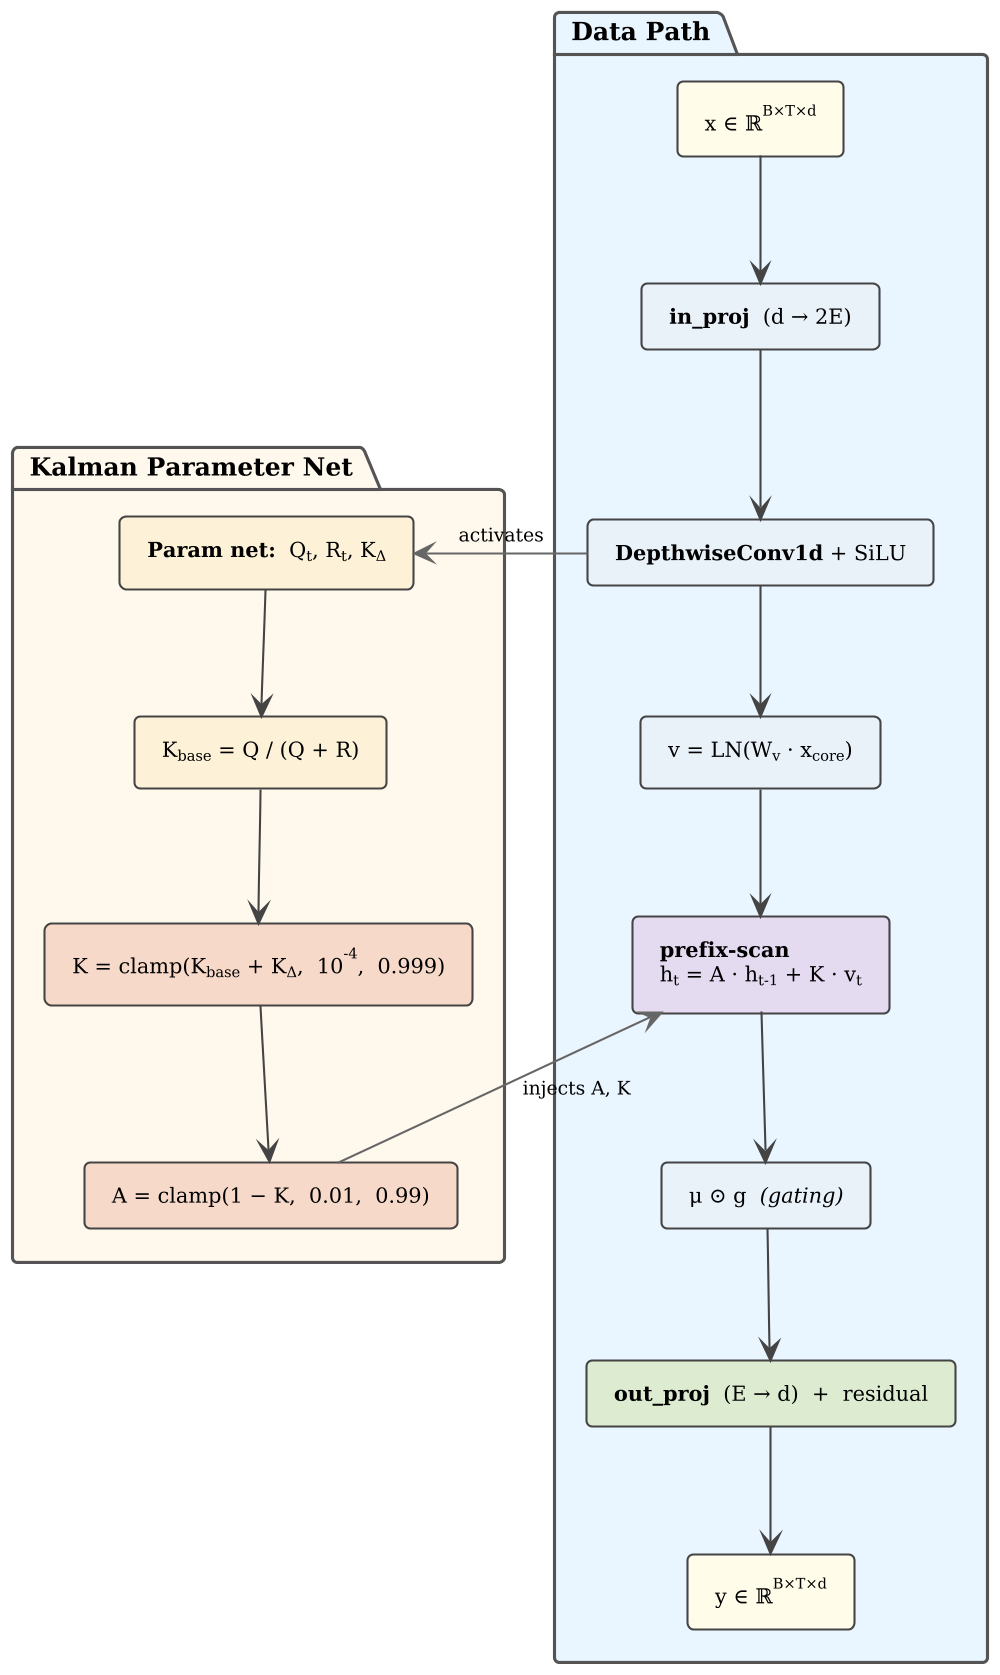
\includegraphics[width=\textwidth, height=0.85\textheight, keepaspectratio]{images/fig08_architecture_en.png}
  \caption{Full data-flow diagram of the KCMamba block. Yellow blocks
           ($Q_\text{net}$, $R_\text{net}$, $K_\text{net}$) learn the Kalman
           statistics. The purple block performs the parallel prefix-scan on GPU
           in $O(\log T)$ synchronisation steps, and green blocks denote
           input/output projections.}
  \label{fig:arch_overview}
\end{figure}

\section{KCMamba Block}
\label{sec:kc_block}

Let the input sequence be $x \in \mathbb{R}^{B \times T \times d}$,
where $B$ is the batch size, $T$ is the sequence length, and $d$ is the
feature dimension.

\subsection{Input Projection and 1D Convolution}

The input is projected into two streams ($x_\text{cw}, x_\text{gate}$) by a
linear layer $W_\text{in} \in \mathbb{R}^{2d_\text{inner} \times d}$,
followed by SiLU gating:
\begin{align}
    [x_\text{cw}, x_\text{gate}] &= W_\text{in} x, \\
    \text{gate} &= \mathrm{SiLU}(x_\text{gate}).
\end{align}
The dual-stream design separates two responsibilities. $x_\text{cw}$ carries
the signal to be filtered by the Kalman layer, while $x_\text{gate}$ learns an
independent amplitude modulation applied at the output stage.
This prevents the gating signal from interfering with the Kalman state dynamics.
$\mathrm{SiLU}(z) = z \cdot \sigma(z)$ is preferred over ReLU because it is
smooth everywhere and allows small negative outputs, which benefits gradient
flow during early training.

Before the global sequential scan, a depthwise 1D convolution ($k=4$ kernel)
on $x_\text{cw}$ integrates short-range temporal context:
\begin{equation}
    x_\text{core} = \mathrm{SiLU}\bigl(\mathrm{Conv1D}(x_\text{cw})\bigr).
\end{equation}
Operating channel-by-channel (depthwise), the convolution adds only
$k \cdot d_\text{inner}$ extra parameters while capturing local temporal
patterns such as short-term momentum and candlestick-level trend direction,
before the Kalman filter processes the full sequence.

\subsection{Kalman Parameter Networks}

Three small two-layer fully connected MLP sub-networks learn the Kalman filter statistics.
$Q_\text{net}$ and $R_\text{net}$ produce the per-step noise variance estimates:
\begin{align}
    Q_t &= \mathrm{softplus}(Q_\text{net}(x_\text{core})) \cdot
           \mathrm{softplus}(q_\text{scale}), \label{eq:Q_net}\\
    R_t &= \mathrm{softplus}(R_\text{net}(x_\text{core})) \cdot
           \mathrm{softplus}(r_\text{scale}). \label{eq:R_net}
\end{align}
$Q_t > 0$ denotes the \emph{process-noise} estimate. When $Q_t$ is large, the
hidden state is expected to change rapidly, so the current measurement
receives more weight.
$R_t > 0$ denotes the \emph{measurement-noise} estimate. A large $R_t$
indicates a noisy observation, causing the model to rely more on its prior state.
The $\mathrm{softplus}$ activation, defined as $\mathrm{softplus}(z) = \ln(1 + e^z) > 0$,
guarantees strict positivity of both quantities, as required by the Kalman
derivation.
The learnable scalars $q_\text{scale}$ and $r_\text{scale}$ set a global
regime bias on top of the per-step outputs.
Initialising $q_\text{scale} = -2.0$ and $r_\text{scale} = 1.5$ gives
$R \gg Q$ at the start, corresponding to $K_\text{base} \approx 0.07$,
meaning strong filtering by default.

A third sub-network, $K_\text{net}$, is also a two-layer fully connected Multi-Layer Perceptron
that provides a direct residual correction to the final gain, described in
Section~\ref{sec:kalman_gain}.
The $Q_\text{net}$/$R_\text{net}$ pair models the slowly evolving noise
regime of the time series, whereas $K_\text{net}$ can react immediately to
fast, content-specific events such as sudden volatility spikes or trend
reversals that the noise-ratio estimate has not yet adapted to.

\subsection{Kalman Gain Computation}
\label{sec:kalman_gain}

The base Kalman gain is derived from the $Q/(Q+R)$ noise ratio, which is the
classical steady-state formula from estimation theory:
\begin{equation}
    K_\text{base,t} = \frac{Q_t}{Q_t + R_t + \varepsilon},
    \label{eq:K_base}
\end{equation}
where $\varepsilon = 10^{-6}$ prevents division by zero.
When $Q \gg R$, meaning the state changes rapidly, $K \to 1$ and the model follows the
current observation closely; when $R \gg Q$, meaning the observations are noisy, $K \to 0$
and the prior state dominates.
This provides an interpretable, physics-grounded prior that aligns with
classical control theory.

A content-dependent correction from $K_\text{net}$ is added to handle rapid
regime changes that the slowly-adapting $Q/R$ ratio may not immediately
capture:
\begin{equation}
    K_t = \mathrm{clamp}\bigl(K_\text{base,t} +
          0.3(\sigma(K_\text{net}(x_\text{core})) - 0.5),\;
          [10^{-4},\; 0.999]\bigr).
    \label{eq:K_final}
\end{equation}
The $-0.5$ shift centres the correction at zero at initialisation, so early
training starts from the $Q/R$ prior rather than a random offset.
The clamp to $[10^{-4},\, 0.999]$ guards against degenerate extremes.
$K_t \approx 0$ would freeze state updates with no new information integrated,
while $K_t \approx 1$ would discard all memory from the previous step.

\subsection{State Update with Parallel Scan}

With forgetting factor $A_t = \mathrm{clamp}(1 - K_t, 0.01, 0.99)$, the
discrete Kalman recurrence is:
\begin{align}
    h_t &= A_t \odot h_{t-1} + K_t \odot v_t, \label{eq:kc_recurrence}\\
    v_t &= \mathrm{LayerNorm}(W_v \, x_\text{core,t}). \nonumber
\end{align}
where $A_t \in (0,1)^{d_\text{inner}}$ is the forgetting factor vector,
with $A_t \to 1$ indicating strong memory and $A_t \to 0$ indicating a strong
update, $\odot$ is the element-wise Hadamard product, $h_{t-1} \in \mathbb{R}^{d_\text{inner}}$
is the previous step's latent state, $v_t$ is the current value vector, and
$W_v \in \mathbb{R}^{d_\text{inner} \times d_\text{inner}}$ is a learnable projection.

Efficient evaluation uses the Blelloch parallel prefix-scan~\cite{blelloch1990prefix}:
\begin{align}
    A_\text{new}[t] &\leftarrow A[t] \cdot A[t-\text{step}], \\
    B_\text{new}[t] &\leftarrow B[t] + A_\text{orig}[t] \cdot B[t-\text{step}],
\end{align}
where $A[t]$ and $B[t]$ are the associative prefix-pair $(a_t, b_t)$: $a_t$ is
the accumulated forgetting factor, $b_t$ is the accumulated input sum.
These are \emph{not} the same as the SSM matrices $A$, $B$.
The stride $\text{step} \in \{1, 2, 4, \ldots, T/2\}$ doubles each pass.
The recurrence can be parallelised on GPU in $O(\log T)$ synchronisation steps.

\begin{figure}[H]
  \centering
  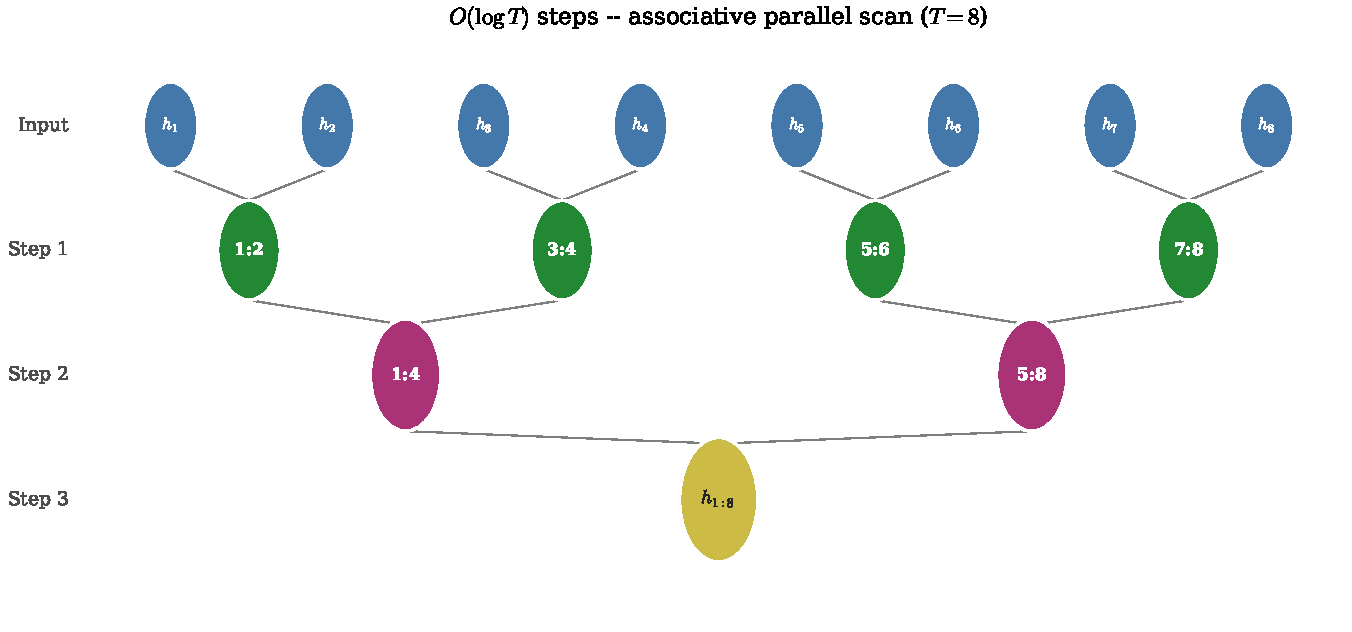
\includegraphics[width=\textwidth]{images/fig09_parallel_scan_en.pdf}
  \caption{Blelloch parallel prefix-scan on a length-8 sequence. Each pass
           combines two elements separated by the current step size, and after
           $\log_2 T = 3$ passes every $h_t$ contains the full context.
           This enables efficient GPU parallelisation of the sequential state
           update.}
  \label{fig:parallel_scan}
\end{figure}

\subsection{Output Projection and Residual Connection}

The Kalman state sequence ($\mu$) is combined with the gate:
\begin{equation}
    y_\text{KC} = W_\text{out}(\mu \odot \text{gate}).
\end{equation}
A scalar-gated residual connection preserves the gradient path:
\begin{equation}
    \text{out} = y_\text{KC} + \sigma(b_\text{res}) \cdot
                 (W_\text{res}\,x - y_\text{KC}),
\end{equation}
where $b_\text{res}$ is a learnable scalar initialised at $-1.0$,
giving $\sigma(b_\text{res}) \approx 0.27$, so the SSM path dominates by default.

\section{KCMamba Stack}
\label{sec:kc_stack}

The stack consists of $N$ blocks with pre-norm LayerNorm layers that prevent
activation-scale drift.
A \emph{multi-scale cross-attention} layer is appended after the final block.
The reason is that Mamba's recurrent dynamics encode recent time steps more
strongly than distant ones in the hidden state.
For long-horizon forecasting, however, slow trends must also be accessible.
The cross-attention queries the current state against the subsampled key/value
set, so both short and long time scales are taken into account:
\begin{equation}
    \text{out}[T] = h[T] + \mathrm{MHA}\bigl(h[T],\; h[{::s}],\; h[{::s}]\bigr),
\end{equation}
where $h[T] \in \mathbb{R}^{1 \times d}$ is the last time step's representation,
serving as the query; $h[{::s}] \in \mathbb{R}^{\lfloor T/s \rfloor \times d}$
is the every-$s$-th subsampled sequence, representing the slower, coarser time
scale as keys and values; and $\mathrm{MHA}(\text{query}, \text{key}, \text{value})$
denotes multi-head cross-attention in the standard
sense~\cite{vaswani2017attention}.

\begin{figure}[H]
  \centering
  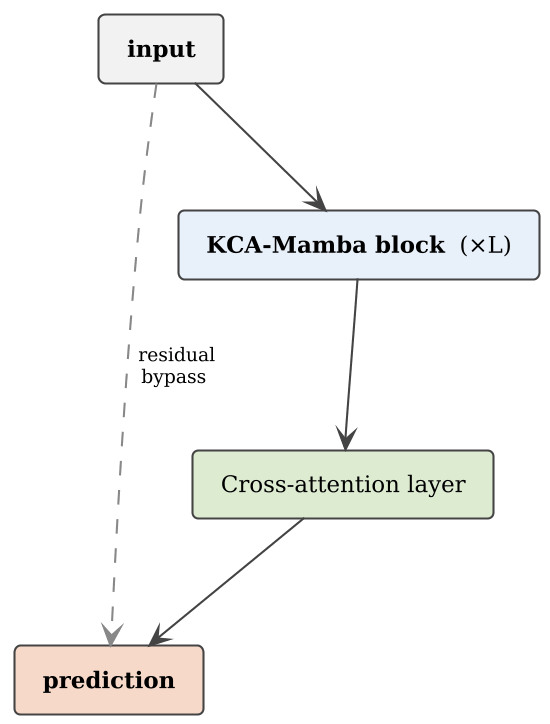
\includegraphics[width=0.55\textwidth, height=0.65\textheight, keepaspectratio]{images/kc_stack_diagram_en.png}
  \caption{KCMamba stack structure. From input to output: input projection,
           2 KC-blocks with LayerNorm, output normalisation, and cross-attention
           for the slow ($s=4$) time scale.}
  \label{fig:stack_diagram}
\end{figure}

\begin{figure}[H]
  \centering
  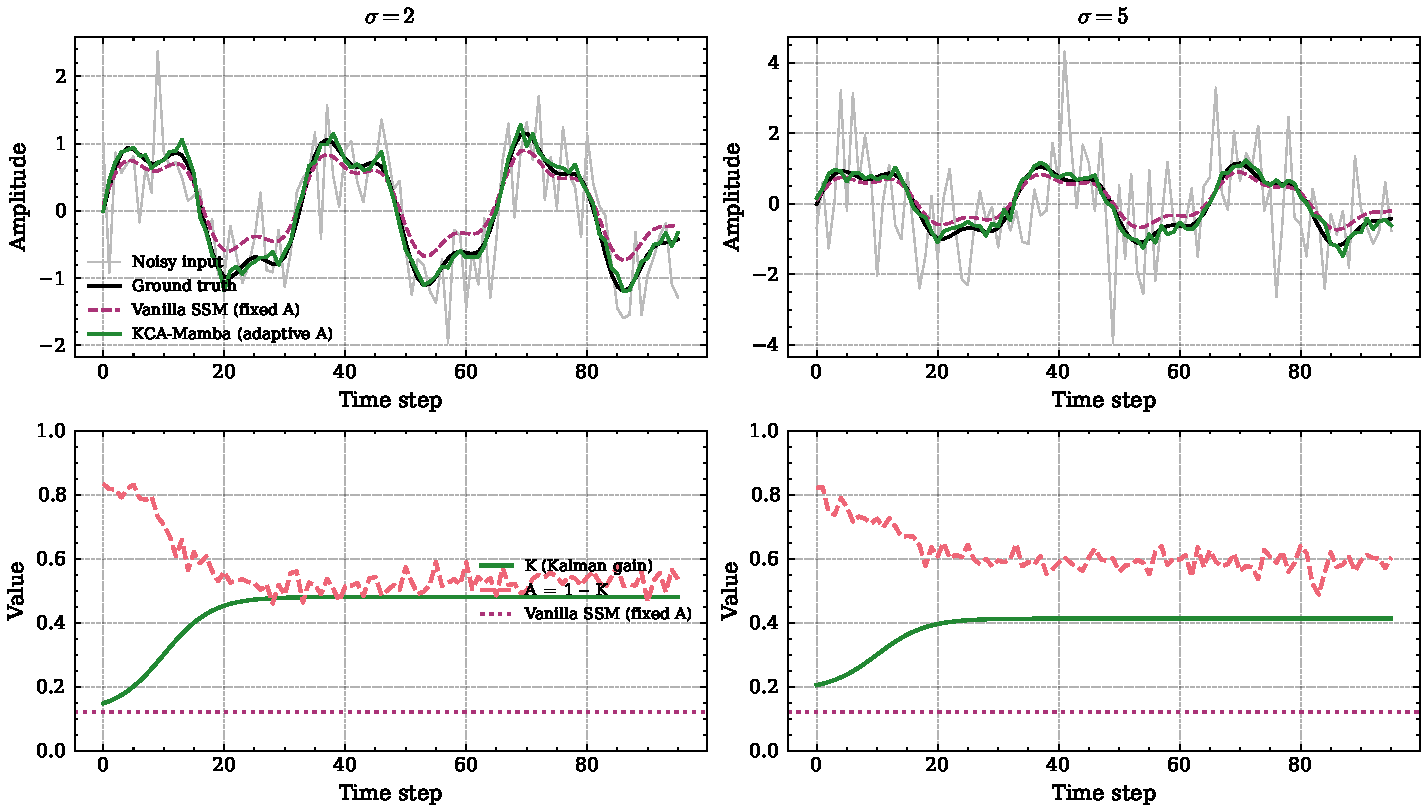
\includegraphics[width=\textwidth]{images/fig11_synth_mamba_en.pdf}
  \caption{Synthetic signal filtering: \textbf{vanilla SSM} (standard Mamba,
           fixed $A$) vs.\ \textbf{KCMamba} (adaptive $K$-gain) at moderate
           ($\sigma=2$) and strong ($\sigma=5$) noise.
           \textit{Top rows:} predicted vs.\ true signal, where KCMamba tracks
           more tightly even under noise.
           \textit{Bottom rows:} learned $K$ values over time.
           Vanilla SSM has a fixed $A$, whereas KCMamba's $A$ adapts with noise level.}
  \label{fig:synth_mamba}
\end{figure}

\begin{figure}[H]
  \centering
  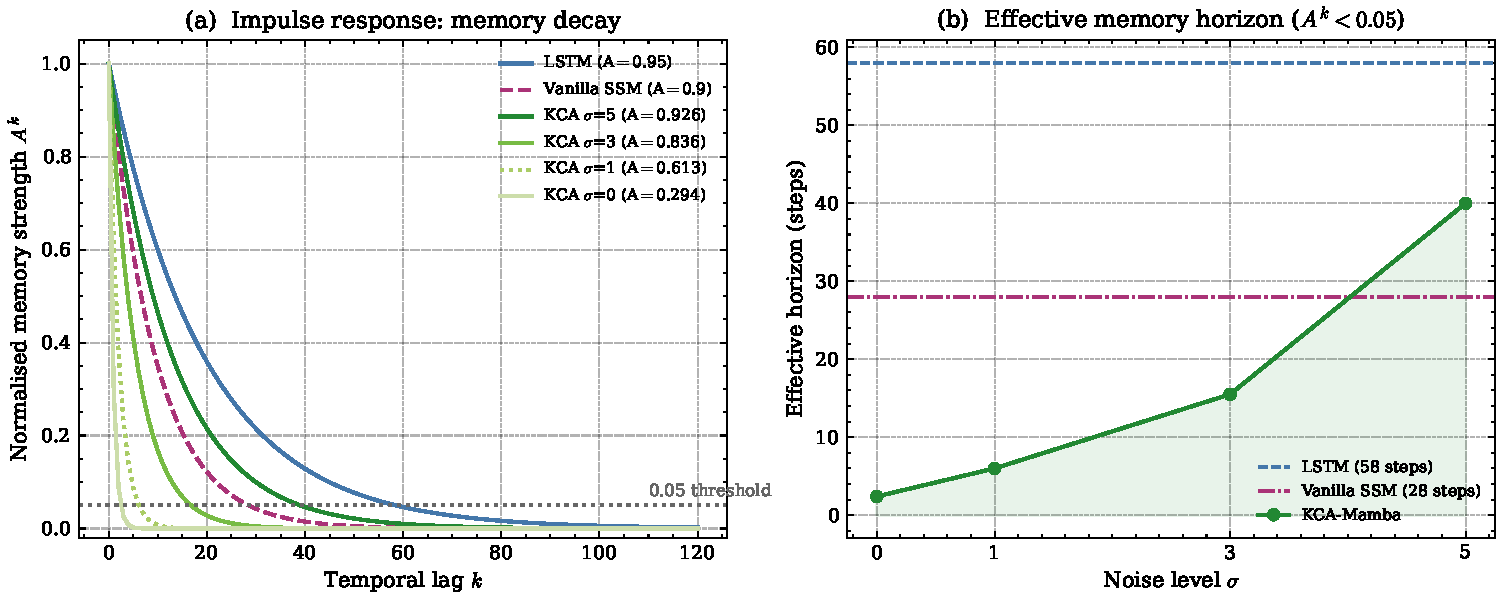
\includegraphics[width=\textwidth]{images/fig13_memory_retention_en.pdf}
  \caption{\textbf{Left:} Impulse-response function: exponential state decay
           $h_k = A^k$ as a function of lag $k$. KCMamba's $A$ grows adaptively
           with noise ($0.294 \to 0.926$), extending the memory horizon.
           \textbf{Right:} Effective memory horizon (number of steps until
           $A^k > 5\%$) vs.\ noise level. LSTM and vanilla SSM have fixed
           horizons, whereas KCMamba automatically extends memory under noise.}
  \label{fig:memory_retention}
\end{figure}

\section{Parameter Complexity}

\begin{table}[H]
    \centering
    \begin{tabular}{|l|r|r|r|}
        \hline
        \textbf{Model} & \textbf{Parameters (k)} & \textbf{Layers} & \textbf{State size} \\
        \hline\hline
        LSTM       & 71{.}7 & 1 & 128 \\
        Fair Mamba & 53{.}2 & 2 & H=4, D=32 \\
        KCMamba  & 46{.}1 & 2 & H=4, D=32 \\
        \hline
    \end{tabular}
    \caption{Parameter complexity of the models used in experiments (medium
             configuration). KCMamba has fewer parameters than Fair Mamba
             because the $Q_\text{net}/R_\text{net}/K_\text{net}$ sub-networks
             redirect resources from the SSM blocks.}
    \label{tab:params}
\end{table}

\section{Comparison with Standard Mamba}

The key architectural difference between \textbf{standard (vanilla) SSM} and
KCMamba lies in how the forgetting factor $A$ is handled.
Standard Mamba~\cite{gu2023mamba} learns $A$ via the time-step $\Delta$, but
this process does not separate signal from noise: $\Delta$ must model both
data structure \emph{and} noise simultaneously.

KCMamba replaces this with an \emph{explicit} $Q/R$ noise domain model:
the $K = Q/(Q+R)$ ratio determines whether to trust the current measurement or
the prior state. At high noise ($\sigma=5$), $K \to 0.073$ and $A = 0.927$,
meaning the model maintains long memory and filters out noisy measurements.
At low noise ($\sigma=0$), $K = 0.706$, so the model follows the current data.

This is demonstrated on the synthetic test in Fig.~\ref{fig:synth_mamba}:
standard SSM uses fixed $A=0.88$ regardless of noise level, while KCMamba
adapts $A$ dynamically (Fig.~\ref{fig:memory_retention}).

\section{System Architecture}
\label{sec:system_arch}

KCMamba is embedded in a hexagonally structured trading system.
Fig.~\ref{fig:system_arch} shows the main components:

\begin{figure}[H]
  \centering
  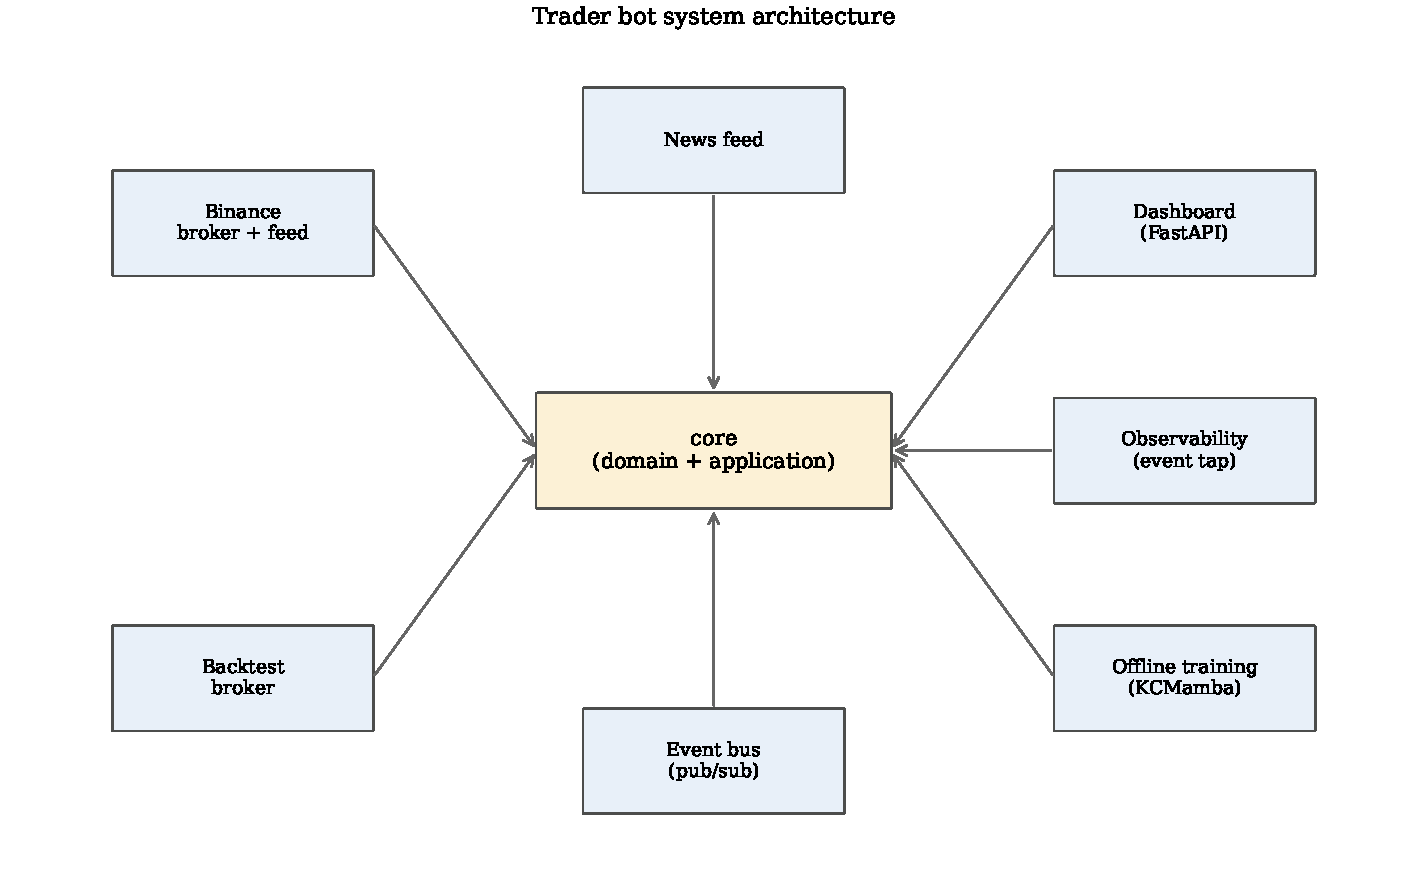
\includegraphics[width=\textwidth]{images/fig14_system_arch_en.pdf}
  \caption{Hexagonal architecture of the KCMamba trading system. The
           \textbf{Core} package contains the TradingEngine
           (pipeline: state estimation $\to$ prediction $\to$ signal $\to$
           risk $\to$ execution), domain models, and application ports.
           External adapters (Infrastructure, Web, Testing, Offline Training,
           Observability, Analytics) communicate with the Core exclusively
           through interfaces ($\texttt{IEventBusPort}$,
           $\texttt{IBrokerGatewayPort}$, etc.).}
  \label{fig:system_arch}
\end{figure}

\section{Module and Class Structure}
\label{sec:module_structure}

The source code is split into four main packages. \texttt{core/} contains all
business logic and holds no references to any adapter. Code in \texttt{adapters/}
accesses the core only through the \texttt{ports.py} interfaces.

\begin{table}[H]
  \centering
  \footnotesize
  \renewcommand{\arraystretch}{1.25}
  \begin{tabular}{|l|p{4.2cm}|p{6.3cm}|}
    \hline
    \textbf{Package} & \textbf{Module / class} & \textbf{Responsibility} \\
    \hline\hline
    \multirow{4}{*}{\texttt{core/domain/}}
      & \texttt{models.py}      & Data types: \texttt{Candle}, \texttt{Position}, \texttt{Order}, \texttt{Fill} \\
      & \texttt{strategy.py}    & \texttt{ThresholdStrategy}: Buy/Sell signal logic,
                                  \texttt{min\_edge}, \texttt{max\_sigma} filters \\
      & \texttt{risk.py}        & \texttt{RiskPolicy}: risk rule set
                                  (MaxQty, Stop-loss, daily loss limit) \\
      & \texttt{events.py}      & Domain events: \texttt{PriceEvent},
                                  \texttt{SignalEvent}, \texttt{FillEvent} \\
    \hline
    \multirow{5}{*}{\texttt{core/application/}}
      & \texttt{engine.py}      & \texttt{TradingEngine}: main pipeline orchestrator,
                                  internal state machine for the trading cycle \\
      & \texttt{execution.py}   & Order assembly, sizing, and dispatch via
                                  \texttt{IBrokerGatewayPort} \\
      & \texttt{ports.py}       & Abstract interfaces:
                                  \texttt{IEventBusPort}, \texttt{IBrokerGatewayPort},
                                  \texttt{IMarketFeedPort}, \texttt{ITimeSourcePort} \\
      & \texttt{stages.py}      & Pipeline stages: \texttt{PredictionStage},
                                  \texttt{SignalStage}, \texttt{RiskStage},
                                  \texttt{ExecutionStage} \\
      & \texttt{stores.py}      & In-memory state: \texttt{PositionStore},
                                  \texttt{SignalStore}, \texttt{EquityStore} \\
    \hline
    \multirow{4}{*}{\texttt{core/ml/}}
      & \texttt{kc\_mamba.py}         & \texttt{KCMambaModel}: PyTorch module,
                                          \texttt{forward(x)} → forecast \\
      & \texttt{mamba\_kalman.py}      & \texttt{KCMambaBlock}: Kalman filter layer,
                                          parallel prefix-scan \\
      & \texttt{services.py}           & \texttt{MLService}: model loading,
                                          online update, forecast cache \\
      & \texttt{feature\_engineering.py} & OHLCV → feature vector transform,
                                            normalisation, sliding window \\
    \hline
    \multirow{5}{*}{\texttt{adapters/}}
      & \texttt{binance\_broker.py}    & \texttt{BinanceBroker}: live order execution
                                          via REST API \\
      & \texttt{binance\_feed.py}      & \texttt{BinanceFeed}: WebSocket price stream,
                                          reconnect logic \\
      & \texttt{event\_bus.py}         & \texttt{InMemoryEventBus}: async
                                          \texttt{asyncio}-based event routing \\
      & \texttt{broker.py} (testing)   & \texttt{PaperBroker}, \texttt{SimulationWallet}:
                                          simulated execution for backtesting \\
      & \texttt{dashboard.py} (web)    & \texttt{DashboardServer}: aiohttp HTTP/WS
                                          server, REST JSON endpoints \\
    \hline
  \end{tabular}
  \caption{Module and class structure of the system. Each class depends only
           on the data types and interfaces of its own package, while cross-package
           dependencies are mediated by the \texttt{ports.py} abstractions.}
  \label{tab:module_structure}
\end{table}
